\documentclass[spanish,letterpaper,oneside]{article}

% Datos del documento
\def\documenttitle {Conversión de fracciones a decimales y viceversa}
\def\documentsubtitle {Temas selectos de matemáticas I}
\def\documentsubject {Actividad 1 · Ficha de trabajo resuelta}
\def\documentauthor {Mtro. Martín Jonathan de la Cruz Muñoz}
\def\coursename {Temas selectos de matemáticas I}
\def\coursecode {PFM02}

% Identidad institucional
\def\universityname {Instituto de Investigación, Innovación y Estudios de Posgrado para la Educación del Estado de Nuevo León}
\def\universityfaculty {Maestría en Aprendizaje y Enseñanza de las Matemáticas}
\def\universitydepartment {Temas selectos de matemáticas I}
\def\universitydepartmentimage {img/iiiepe/marca-iiiepe.png}
\def\universitydepartmentimagecfg {height=1.75cm}
\def\universitylocation {Monterrey, Nuevo León}
\def\studentfullname {Mtro. Martín Jonathan de la Cruz Muñoz}
\def\studentid {00874}
\def\studentemail {martin.delacruz@campus.iiiepe.edu.mx}
\def\programperiod {1er tetramestre, marzo--julio de 2026}
\def\programmodality {Modalidad presencial}
\def\programshort {MAEM}

\def\authortable {
  \begin{tabular}{ll}
    \textbf{Alumno:} & \studentfullname \\
    Matrícula: & \studentid \\
    Correo institucional: & \studentemail \\
    Unidad: & \coursename \\
    Programa: & \programshort \\
    Periodo: & \programperiod \\
    & \\
    \multicolumn{2}{l}{Fecha de realización: 13 de octubre de 2026} \\
    \multicolumn{2}{l}{\universitylocation}
  \end{tabular}
}

\input{template}

\usepackage{helvet}
\renewcommand{\familydefault}{\sfdefault}
\usepackage{array}
\usepackage{longtable}
\usepackage{pdflscape}
\usepackage{tikz}
\usepackage[most]{tcolorbox}
\usetikzlibrary{arrows.meta,positioning,calc,fit,backgrounds}

\definecolor{iiiepeNavy}{HTML}{163B5C}
\definecolor{iiiepeBlue}{HTML}{1F6F9F}
\definecolor{iiiepeAqua}{HTML}{20B7A8}
\definecolor{iiiepeOrange}{HTML}{F28C28}
\definecolor{iiiepePaper}{HTML}{F6F8F7}
\definecolor{iiiepeInk}{HTML}{1E2A32}
\def\portraittitlecolor {iiiepeNavy}
\setcitestyle{authoryear,open={(},close={)}}

\newcommand{\insertcoverwatermark}{%
  \AddToShipoutPictureBG*{%
    \begin{tikzpicture}[remember picture,overlay]
      \node[opacity=.09,inner sep=0pt] at (current page.center)
      {\includegraphics[width=.58\paperwidth]{img/iiiepe/logo-puntos.png}};
    \end{tikzpicture}%
  }%
}

\newtcolorbox{reportelecturabox}[1][]{%
  enhanced,breakable,
  colback=iiiepePaper,colframe=iiiepeNavy,
  boxrule=1pt,leftrule=4pt,arc=2pt,
  left=8pt,right=8pt,top=6pt,bottom=6pt,
  before skip=6pt,after skip=10pt,
  fonttitle=\bfseries\color{white},coltitle=white,
  colbacktitle=iiiepeNavy,
  attach boxed title to top left={xshift=8pt,yshift=-2pt},
  boxed title style={colback=iiiepeNavy,colframe=iiiepeNavy,arc=1pt},
  title={Reporte de lectura},#1}

\newtcolorbox{fichalecturabox}[1][]{%
  enhanced,breakable,
  colback=iiiepeAqua!7,colframe=iiiepeAqua!70!iiiepeNavy,
  boxrule=.6pt,arc=1pt,
  left=7pt,right=7pt,top=4pt,bottom=4pt,
  fontupper=\small,before upper={\setstretch{1.0}},
  fonttitle=\bfseries\color{iiiepeNavy},coltitle=iiiepeNavy,
  colbacktitle=iiiepeAqua!7,
  title={Ficha de la lectura},#1}



\usepackage{tabularx,colortbl,pgfplots,enumitem,needspace}\pgfplotsset{compat=1.18}\definecolor{iiiepePale}{HTML}{EEF5F8}
\setlength{\parskip}{5pt}\setlength{\parindent}{0pt}
\begin{document}\insertcoverwatermark\templatePortrait\templatePagecfg\templateFinalcfg\fancyfoot{}\fancyfoot[L]{\scriptsize IIIEPE · MAEM}\fancyfoot[C]{\scriptsize\thepage}\fancyfoot[R]{\scriptsize Actividad 1}\setstretch{1.3}\raggedbottom
\section{Representar la misma cantidad de dos maneras}
Convertir una fracción a decimal consiste en efectuar la división del numerador entre el denominador. El valor no cambia; cambia su representación. Una fracción irreducible tiene decimal finito si su denominador solo contiene factores 2 y 5. En los demás casos aparece un período. En mantenimiento y mecatrónica, esta equivalencia permite interpretar una medida en pulgadas y compararla con un catálogo decimal sin redondear antes de tiempo.
\[
\frac{a}{b}=a\div b,\qquad n\frac{a}{b}=n+\frac{a}{b},\qquad b\ne0.
\]

\begin{center}
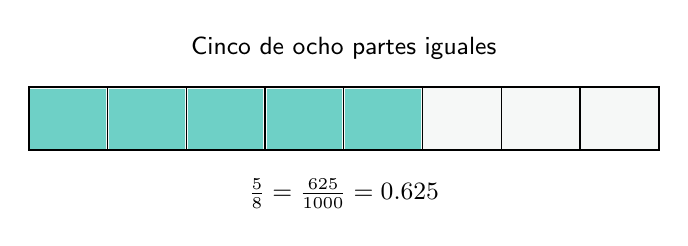
\begin{tikzpicture}[x=1cm,y=1cm,font=\small]
\foreach \i in {0,...,7}{\draw[fill=iiiepePaper] (\i,0) rectangle +(1,.8);}\foreach \i in {0,...,4}{\fill[iiiepeAqua!65] (\i+.02,.02) rectangle +( .96,.76);}\draw[thick] (0,0) rectangle (8,.8);
\node at (4,1.3){Cinco de ocho partes iguales};\node at (4,-.55){$\frac58=\frac{625}{1000}=0.625$};\end{tikzpicture}
\end{center}
\section{Ejercicios de la ficha oficial resueltos}
\subsection*{Fracciones decimales}


{\small\setstretch{1.1}\renewcommand{\arraystretch}{1.25}
\begin{longtable}{|>{\raggedright\arraybackslash}p{\dimexpr0.5\linewidth-2\tabcolsep-2\arrayrulewidth\relax}|>{\raggedright\arraybackslash}p{\dimexpr0.5\linewidth-2\tabcolsep-2\arrayrulewidth\relax}|}\hline
\rowcolor{iiiepePale} \textbf{Expresión} & \textbf{Procedimiento y resultado} \\\hline
\endfirsthead
\hline
\rowcolor{iiiepePale} \textbf{Expresión} & \textbf{Procedimiento y resultado} \\\hline
\endhead
$\frac{3}{10}$ & $3\div 10=0.3$ \\\hline
$\frac{8}{10}$ & $8\div 10=0.8$ \\\hline
$\frac{1}{10}$ & $1\div 10=0.1$ \\\hline
$\frac{6}{10}$ & $6\div 10=0.6$ \\\hline
$\frac{17}{10}$ & $17\div 10=1.7$ \\\hline
$\frac{75}{100}$ & $75\div 100=0.75$ \\\hline
$\frac{25}{100}$ & $25\div 100=0.25$ \\\hline
$\frac{80}{100}$ & $80\div 100=0.8$ \\\hline
\end{longtable}}



{\small\setstretch{1.1}\renewcommand{\arraystretch}{1.25}
\begin{longtable}{|>{\raggedright\arraybackslash}p{\dimexpr0.5\linewidth-2\tabcolsep-2\arrayrulewidth\relax}|>{\raggedright\arraybackslash}p{\dimexpr0.5\linewidth-2\tabcolsep-2\arrayrulewidth\relax}|}\hline
\rowcolor{iiiepePale} \textbf{Expresión} & \textbf{Procedimiento y resultado} \\\hline
\endfirsthead
\hline
\rowcolor{iiiepePale} \textbf{Expresión} & \textbf{Procedimiento y resultado} \\\hline
\endhead
$\frac{50}{100}$ & $50\div 100=0.5$ \\\hline
$\frac{375}{100}$ & $375\div 100=3.75$ \\\hline
$\frac{125}{1000}$ & $125\div 1000=0.125$ \\\hline
$\frac{375}{1000}$ & $375\div 1000=0.375$ \\\hline
$\frac{700}{1000}$ & $700\div 1000=0.7$ \\\hline
$\frac{615}{1000}$ & $615\div 1000=0.615$ \\\hline
$\frac{4455}{1000}$ & $4455\div 1000=4.455$ \\\hline
$\frac{45}{1000}$ & $45\div 1000=0.045$ \\\hline
\end{longtable}}



{\small\setstretch{1.1}\renewcommand{\arraystretch}{1.25}
\begin{longtable}{|>{\raggedright\arraybackslash}p{\dimexpr0.5\linewidth-2\tabcolsep-2\arrayrulewidth\relax}|>{\raggedright\arraybackslash}p{\dimexpr0.5\linewidth-2\tabcolsep-2\arrayrulewidth\relax}|}\hline
\rowcolor{iiiepePale} \textbf{Expresión} & \textbf{Procedimiento y resultado} \\\hline
\endfirsthead
\hline
\rowcolor{iiiepePale} \textbf{Expresión} & \textbf{Procedimiento y resultado} \\\hline
\endhead
$\frac{4}{100}$ & $4\div 100=0.04$ \\\hline
$\frac{815}{10}$ & $815\div 10=81.5$ \\\hline
$\frac{1}{1000}$ & $1\div 1000=0.001$ \\\hline
$\frac{5}{100}$ & $5\div 100=0.05$ \\\hline
\end{longtable}}

\subsection*{Fracciones propias}


{\small\setstretch{1.1}\renewcommand{\arraystretch}{1.25}
\begin{longtable}{|>{\raggedright\arraybackslash}p{\dimexpr0.5\linewidth-2\tabcolsep-2\arrayrulewidth\relax}|>{\raggedright\arraybackslash}p{\dimexpr0.5\linewidth-2\tabcolsep-2\arrayrulewidth\relax}|}\hline
\rowcolor{iiiepePale} \textbf{Expresión} & \textbf{Procedimiento y resultado} \\\hline
\endfirsthead
\hline
\rowcolor{iiiepePale} \textbf{Expresión} & \textbf{Procedimiento y resultado} \\\hline
\endhead
$\frac{3}{4}$ & $3\div 4=0.75$ \\\hline
$\frac{4}{5}$ & $4\div 5=0.8$ \\\hline
$\frac{1}{8}$ & $1\div 8=0.125$ \\\hline
$\frac{3}{10}$ & $3\div 10=0.3$ \\\hline
$\frac{5}{16}$ & $5\div 16=0.3125$ \\\hline
$\frac{4}{8}$ & $4\div 8=0.5$ \\\hline
$\frac{4}{25}$ & $4\div 25=0.16$ \\\hline
$\frac{18}{50}$ & $18\div 50=0.36$ \\\hline
\end{longtable}}

\subsection*{Fracciones impropias}


{\small\setstretch{1.1}\renewcommand{\arraystretch}{1.25}
\begin{longtable}{|>{\raggedright\arraybackslash}p{\dimexpr0.5\linewidth-2\tabcolsep-2\arrayrulewidth\relax}|>{\raggedright\arraybackslash}p{\dimexpr0.5\linewidth-2\tabcolsep-2\arrayrulewidth\relax}|}\hline
\rowcolor{iiiepePale} \textbf{Expresión} & \textbf{Procedimiento y resultado} \\\hline
\endfirsthead
\hline
\rowcolor{iiiepePale} \textbf{Expresión} & \textbf{Procedimiento y resultado} \\\hline
\endhead
$\frac{6}{4}$ & $6\div 4=1.5$ \\\hline
$\frac{8}{5}$ & $8\div 5=1.6$ \\\hline
$\frac{13}{8}$ & $13\div 8=1.625$ \\\hline
$\frac{10}{4}$ & $10\div 4=2.5$ \\\hline
$\frac{21}{6}$ & $21\div 6=3.5$ \\\hline
$\frac{17}{4}$ & $17\div 4=4.25$ \\\hline
$\frac{23}{20}$ & $23\div 20=1.15$ \\\hline
$\frac{34}{5}$ & $34\div 5=6.8$ \\\hline
\end{longtable}}

\subsection*{Números mixtos}


{\small\setstretch{1.1}\renewcommand{\arraystretch}{1.25}
\begin{longtable}{|>{\raggedright\arraybackslash}p{\dimexpr0.5\linewidth-2\tabcolsep-2\arrayrulewidth\relax}|>{\raggedright\arraybackslash}p{\dimexpr0.5\linewidth-2\tabcolsep-2\arrayrulewidth\relax}|}\hline
\rowcolor{iiiepePale} \textbf{Expresión} & \textbf{Procedimiento y resultado} \\\hline
\endfirsthead
\hline
\rowcolor{iiiepePale} \textbf{Expresión} & \textbf{Procedimiento y resultado} \\\hline
\endhead
$7+\frac{2}{5}$ & $7+0.4=7.4$ \\\hline
$3+\frac{1}{4}$ & $3+0.25=3.25$ \\\hline
$12+\frac{17}{20}$ & $12+0.85=12.85$ \\\hline
$1+\frac{9}{10}$ & $1+0.9=1.9$ \\\hline
$5+\frac{7}{8}$ & $5+0.875=5.875$ \\\hline
$6+\frac{13}{40}$ & $6+0.325=6.325$ \\\hline
$2+\frac{8}{5}$ & $2+1.6=3.6$ \\\hline
$4+\frac{10}{8}$ & $4+1.25=5.25$ \\\hline
\end{longtable}}

Los incisos $2\frac85$ y $4\frac{10}{8}$ se interpretan como sumas, aunque su parte fraccionaria sea impropia. Sus formas mixtas convencionales son $3\frac35$ y $5\frac14$, respectivamente.\subsection*{Decimales periódicos}


{\small\setstretch{1.1}\renewcommand{\arraystretch}{1.25}
\begin{longtable}{|>{\raggedright\arraybackslash}p{\dimexpr0.5\linewidth-2\tabcolsep-2\arrayrulewidth\relax}|>{\raggedright\arraybackslash}p{\dimexpr0.5\linewidth-2\tabcolsep-2\arrayrulewidth\relax}|}\hline
\rowcolor{iiiepePale} \textbf{Expresión} & \textbf{Procedimiento y resultado} \\\hline
\endfirsthead
\hline
\rowcolor{iiiepePale} \textbf{Expresión} & \textbf{Procedimiento y resultado} \\\hline
\endhead
$\frac13$ & $0.\overline3$ \\\hline
$\frac79$ & $0.\overline7$ \\\hline
$2+\frac7{11}$ & $2.\overline{63}$ \\\hline
$\frac{13}6$ & $2.1\overline6$ \\\hline
$5+\frac4{15}$ & $5.2\overline6$ \\\hline
$\frac{20}{11}$ & $1.\overline{81}$ \\\hline
$\frac6{27}$ & $\frac29=0.\overline2$ \\\hline
$\frac{22}{90}$ & $\frac{11}{45}=0.2\overline4$ \\\hline
\end{longtable}}

\subsection*{Decimales finitos a fracción}
Se escribe el decimal sobre $10^n$, donde $n$ es el número de cifras decimales, y se simplifica mediante el máximo común divisor.
\subsection*{Resultados exactos}


{\small\setstretch{1.1}\renewcommand{\arraystretch}{1.25}
\begin{longtable}{|>{\raggedright\arraybackslash}p{\dimexpr0.5\linewidth-2\tabcolsep-2\arrayrulewidth\relax}|>{\raggedright\arraybackslash}p{\dimexpr0.5\linewidth-2\tabcolsep-2\arrayrulewidth\relax}|}\hline
\rowcolor{iiiepePale} \textbf{Expresión} & \textbf{Procedimiento y resultado} \\\hline
\endfirsthead
\hline
\rowcolor{iiiepePale} \textbf{Expresión} & \textbf{Procedimiento y resultado} \\\hline
\endhead
$1.6$ & $\frac{16}{10}=\frac{8}{5}$ \\\hline
$0.525$ & $\frac{525}{1000}=\frac{21}{40}$ \\\hline
$0.025$ & $\frac{25}{1000}=\frac{1}{40}$ \\\hline
$0.75$ & $\frac{75}{100}=\frac{3}{4}$ \\\hline
$34.5$ & $\frac{345}{10}=\frac{69}{2}$ \\\hline
$1.5$ & $\frac{15}{10}=\frac{3}{2}$ \\\hline
$0.17$ & $\frac{17}{100}=\frac{17}{100}$ \\\hline
$2.05$ & $\frac{205}{100}=\frac{41}{20}$ \\\hline
\end{longtable}}

\subsection*{Decimales periódicos a fracción}
Si hay $m$ cifras no periódicas y $n$ cifras de período, se multiplican dos copias del número por $10^{m+n}$ y $10^m$ y se restan. Así desaparece la cola infinita; no se aproxima el número.
\subsection*{Eliminación del período}


{\small\setstretch{1.1}\renewcommand{\arraystretch}{1.25}
\begin{longtable}{|>{\raggedright\arraybackslash}p{\dimexpr0.5\linewidth-2\tabcolsep-2\arrayrulewidth\relax}|>{\raggedright\arraybackslash}p{\dimexpr0.5\linewidth-2\tabcolsep-2\arrayrulewidth\relax}|}\hline
\rowcolor{iiiepePale} \textbf{Expresión} & \textbf{Procedimiento y resultado} \\\hline
\endfirsthead
\hline
\rowcolor{iiiepePale} \textbf{Expresión} & \textbf{Procedimiento y resultado} \\\hline
\endhead
$0.\overline{18}$ & $\frac{18}{99}=\frac2{11}$ \\\hline
$0.\overline7$ & $\frac79$ \\\hline
$2.1\overline6$ & $\frac{216-21}{90}=\frac{13}6$ \\\hline
$0.5\overline3$ & $\frac{53-5}{90}=\frac8{15}$ \\\hline
$0.82\overline1$ & $\frac{821-82}{900}=\frac{739}{900}$ \\\hline
$1.4\overline{67}$ & $\frac{1467-14}{990}=\frac{1453}{990}$ \\\hline
$0.\overline{009}$ & $\frac9{999}=\frac1{111}$ \\\hline
$5.8\overline{72}$ & $\frac{5872-58}{990}=\frac{323}{55}$ \\\hline
\end{longtable}}

Por ejemplo, si $x=2.1\overline6$, entonces $100x=216.\overline6$ y $10x=21.\overline6$. Al restar, $90x=195$ y $x=13/6$.\section{Situaciones contextualizadas}

{\small\setstretch{1.1}\renewcommand{\arraystretch}{1.25}
\begin{longtable}{|>{\raggedright\arraybackslash}p{\dimexpr0.22\linewidth-2\tabcolsep-2\arrayrulewidth\relax}|>{\raggedright\arraybackslash}p{\dimexpr0.78\linewidth-2\tabcolsep-2\arrayrulewidth\relax}|}\hline
\rowcolor{iiiepePale} \textbf{Situación} & \textbf{Solución e interpretación} \\\hline
\endfirsthead
\hline
\rowcolor{iiiepePale} \textbf{Situación} & \textbf{Solución e interpretación} \\\hline
\endhead
1 & CDMX: $9/100=0.09$; Estado de México y Coahuila: $14/100=0.14$; Chiapas: $32/100=0.32$; Oaxaca y Michoacán: $29/100=0.29$. Se convierten los datos históricos del enunciado, sin tratarlos como estadísticas actuales. \\\hline
2 & $4+5/12=4.41\overline6$ años. La fracción usa 12 meses por año; no representa $4.5$ años. \\\hline
3 & Falta $1-7/18=11/18=0.6\overline1$ de la parcela. \\\hline
4 & $0.16=16/100=4/25$. \\\hline
5 & $3.790=3790/1000=379/100$ litros, usando la equivalencia dada en la ficha. \\\hline
6 & $11/16=0.6875$ pulgadas. \\\hline
7 & Árbol: $329/100$ m; fruta: $6/100$ m; edificio: $159/10$ m; mariposa: $53/1000$ m. \\\hline
8 & La báscula indica $0.85$ kg: $85/100=17/20$ kg. \\\hline
\end{longtable}}



{\small\setstretch{1.1}\renewcommand{\arraystretch}{1.25}
\begin{longtable}{|>{\raggedright\arraybackslash}p{\dimexpr0.22\linewidth-2\tabcolsep-2\arrayrulewidth\relax}|>{\raggedright\arraybackslash}p{\dimexpr0.78\linewidth-2\tabcolsep-2\arrayrulewidth\relax}|}\hline
\rowcolor{iiiepePale} \textbf{Situación} & \textbf{Solución e interpretación} \\\hline
\endfirsthead
\hline
\rowcolor{iiiepePale} \textbf{Situación} & \textbf{Solución e interpretación} \\\hline
\endhead
9 & $7/40=175/1000=0.175$ mm; se selecciona ese grosor. \\\hline
10 & Interpretando la figura como cuadrado de lado $2.2$ cm: $P=4(2.2)=8.8=44/5$ cm. Si no fuera un cuadrado, una sola medida no permitiría determinar el perímetro. \\\hline
11 & Diámetros: $1/3=0.\overline3$ m; $5/6=0.8\overline3$ m; $3/11=0.\overline{27}$ m; $17/12=1.41\overline6$ m. \\\hline
12 & $P=2(2.80+3/5)=2(3.4)=6.8$ cm. \\\hline
\end{longtable}}

\section{Por qué funcionan las conversiones}
\subsection{División y valor posicional}
Para convertir $11/16$, se inicia con $11<16$. Al expresar el residuo en décimos, $110=16(6)+14$; en centésimos, $140=16(8)+12$; en milésimos, $120=16(7)+8$; y en diezmilésimos, $80=16(5)$. Por ello, $11/16=0.6875$. La comprobación inversa es $6875/10000=11/16$. Este recorrido permite localizar una cifra errónea sin depender de una calculadora.
\subsection{Una cola infinita no es una aproximación finita}
Si $x=0.\overline{18}$, entonces $100x=18.\overline{18}$; al restar, $99x=18$ y $x=2/11$. En cambio, $0.18=18/100=9/50$. Las dos cantidades difieren aunque coincidan sus primeras cifras. Para $x=0.82\overline1$, $1000x=821.\overline1$ y $100x=82.\overline1$; así $900x=739$ y $x=739/900$. La cantidad de ceros y nueves del denominador proviene de esta resta, no de una regla sin fundamento.
\subsection{Transferencia técnica}
Una tolerancia didáctica de $\pm1/32$ de pulgada equivale a $\pm0.03125$ pulgadas. Si un catálogo muestra tres decimales, habría que declarar el redondeo y comprobar si su precisión es compatible con la decisión. Este ejemplo no prescribe una tolerancia industrial: permite discutir la diferencia entre valor exacto, escritura disponible y criterio de aceptación.
\section{Secuencia de aplicación y evaluación}
Convertir racionales con equivalencias exactas. La duración propuesta es de 60 minutos, ajustable al diagnóstico y a los recursos. Esta planeación sigue la progresión de los recursos institucionales (IIIEPE, 2026); los tiempos y apoyos son decisiones de codiseño, no datos de una aplicación ya realizada.

{\small\setstretch{1.1}\renewcommand{\arraystretch}{1.25}
\begin{longtable}{|>{\raggedright\arraybackslash}p{\dimexpr0.23\linewidth-2\tabcolsep-2\arrayrulewidth\relax}|>{\raggedright\arraybackslash}p{\dimexpr0.49\linewidth-2\tabcolsep-2\arrayrulewidth\relax}|>{\raggedright\arraybackslash}p{\dimexpr0.28\linewidth-2\tabcolsep-2\arrayrulewidth\relax}|}\hline
\rowcolor{iiiepePale} \textbf{Fase y tiempo} & \textbf{Actividad y mediación} & \textbf{Evidencia} \\\hline
\endfirsthead
\hline
\rowcolor{iiiepePale} \textbf{Fase y tiempo} & \textbf{Actividad y mediación} & \textbf{Evidencia} \\\hline
\endhead
1. Antecedentes (8 min) & Estimar una medida de herramienta y registrar su escritura fraccionaria. & Predicción individual y pregunta. \\\hline
2. Explicación (12 min) & Reconstruir división, valor posicional y eliminación del período. & Plan explicado y criterios. \\\hline
3. Práctica (20 min) & Resolver dos conversiones y comprobarlas en sentido inverso. & Registro o procedimiento trazable. \\\hline
4. Evaluación (12 min) & Distinguir un decimal finito de uno periódico en un caso nuevo. & Argumento con comprobación. \\\hline
5. Retroalimentación (8 min) & Corregir una equivalencia y explicar la primera diferencia detectada. & Versión revisada y justificación. \\\hline
\end{longtable}}
\subsection{Criterios observables y retroalimentación}

{\small\setstretch{1.1}\renewcommand{\arraystretch}{1.25}
\begin{longtable}{|>{\raggedright\arraybackslash}p{\dimexpr0.22\linewidth-2\tabcolsep-2\arrayrulewidth\relax}|>{\raggedright\arraybackslash}p{\dimexpr0.4\linewidth-2\tabcolsep-2\arrayrulewidth\relax}|>{\raggedright\arraybackslash}p{\dimexpr0.38\linewidth-2\tabcolsep-2\arrayrulewidth\relax}|}\hline
\rowcolor{iiiepePale} \textbf{Criterio} & \textbf{Evidencia de logro} & \textbf{Acción si necesita apoyo} \\\hline
\endfirsthead
\hline
\rowcolor{iiiepePale} \textbf{Criterio} & \textbf{Evidencia de logro} & \textbf{Acción si necesita apoyo} \\\hline
\endhead
Valor exacto y aproximación & Explica valor exacto y aproximación con un caso de la actividad. & Pedir una representación concreta y contrastar dos casos. \\\hline
Procedimiento de conversión & Conserva procedimiento de conversión en el desarrollo y justifica sus pasos. & Modelar un paso, retirar gradualmente la ayuda y solicitar otro caso. \\\hline
Comprobación inversa & Utiliza comprobación inversa para contrastar una respuesta o representación. & Comparar la evidencia inicial y la corregida con una pregunta específica. \\\hline
Interpretación de unidades & Relaciona interpretación de unidades con la conclusión y un límite del problema. & Solicitar una comprobación independiente y un caso de transferencia. \\\hline
\end{longtable}}
El instrumento es una propuesta docente. Cada criterio se registra como logrado con autonomía, logrado con apoyo o aún no demostrado; no se asigna una calificación observada sin aplicar la actividad. En la coevaluación, un compañero verifica un criterio y formula una pregunta; en la autoevaluación, el estudiante explica una corrección; el docente contrasta ambas evidencias y decide el siguiente apoyo.\subsection{Participación y apoyos}
La inclusión se concreta en alternativas de representación y de acceso; el pensamiento crítico, en justificar y contrastar. Los roles de cálculo, registro y explicación se rotan para que todos produzcan una evidencia individual. Quien necesita apoyo dispone de un ejemplo parcial y preguntas graduadas; quien ya domina el procedimiento analiza un contraejemplo o cambia una condición. Estas acciones deben observarse durante la aplicación para valorar su funcionamiento.

\section{Reflexión pedagógica y evaluación}
Propongo iniciar con llaves españolas, espesores y diámetros de ruedas, porque permiten preguntar por el significado de una medida antes de ejecutar una conversión. Después solicitaría dos representaciones del mismo valor y una comprobación inversa. La precisión técnica se conserva, pero el error deja de ser una descalificación: indica si conviene revisar valor posicional, división o período.
La evidencia de logro sería que el estudiante explique por qué $0.5=1/2$, distinga $0.33$ de $0.\overline3$ y mantenga las unidades. Retroalimentaría la primera diferencia entre su procedimiento y una equivalencia válida; después le pediría corregir un inciso y resolver otro nuevo. La autoevaluación de participación y desempeño debe completarse a partir del trabajo efectivamente realizado.

\needspace{5\baselineskip}\section*{Referencias}
{\setstretch{1.15}\setlength{\parskip}{6pt}
\par\hangindent=1.27cm\hangafter=1  IIIEPE. (2026). \textit{Sesión 01: Conversión de fracciones a decimales y viceversa}. Ficha de Temas selectos de matemáticas I, EVA posgrado.
\par\hangindent=1.27cm\hangafter=1  Secretaría de Educación Pública. (2024). \textit{Programa de estudio para la educación secundaria: Programa sintético de la Fase 6}. SEP.
}

\end{document}
